%{

{
\cleardoublepage

%\pagestyle{plain}      % ← отключаем fancy-стиль
%\thispagestyle{plain}  % ← на текущей (первой) странице эпилога

\phantomsection

\fancyhead[LE]{\fancyplain{}{}}
\fancyhead[RO]{\fancyplain{}{}}

%\pagestyle{empty}
%\thispagestyle{mystyle}
%\addtocontents{toc}{\vspace{-5mm}}
\bookmarksetup{startatroot}% this is it
%\addtocontents{toc}{\vspace{1\baselineskip}}
\addcontentsline{toc}{chapter}{Эпилог}
%\pdfbookmark[-1]{Эпилог}{epilog}
%\addtocontents{toc}{\vspace{-6mm}}
\section*{Эпилог}
%\chapter*{Эпилог}

%Перевалило за полночь. Шурик сидел у себя на~кухне в~домашних штанах и майке, лениво потягивая из коньячного бокала 7\sdash летний ром. Жена у плиты хлопотала блинчики сыну на утро. Шурик задумчиво рассматривал жену сзади, любуясь, будто бы в первый раз, формами. Их сын мирно посапывал в кроватке. В мире творился трындец. Жизнь~продолжалась$\ldots$

Перевалило за полночь. Шурик сидел у себя на~кухне в~домашних штанах и майке, лениво потягивая из коньячного бокала. Жена у плиты хлопотала блинчики сыну на~утро. Их сын мирно посапывал в~кроватке. Шурик отрешённо и~задумчиво рассматривал жену сзади, любуясь, будто бы в~первый раз, формами. 

Никаких его проблем сплав, поход, конечно же не~решил, да и не мог решить. Но отдых, тем не менее, удался на славу\mdash это Шурик мог утверждать с уверенностью. Они оторвались с пацанами по полной программе, б\'{о}льшего и~желать грешновато на одно путешествие двухнедельное\mdash и в Старой Ладоге побывали, и на Киваче, и пороги взяли, и~поробинзонили, и рыбы наелись карельской, наговорились обо всём и вся, напитались атмосферой Карелии.

Это путешествие, как и любой другой их вояж по~рекам, выключило команду из привычного опостылевшего ритма городской жизни и заставило пережить бурю ярких эмоций и~целую гамму чувств, понять которые под силу только тем, кто хоть раз был в походе. Это ли не смысл отдыха? Смена деятельности, порой такая вот <<ударная>>. Мышцы рук к~концу похода уже полностью адаптировались и~перестали ныть от весла, втянулись, что называется. Тут~бы~плыть и~плыть дальше, ан~нет, пожалуйте обратно в~<<каменные~джунгли>>$\ldots$

Жена что\sdash то говорила ему, он на автомате отвечал, а~всеми мыслями был ещё там, на реке. Там он был Адмиралом, Командиром, там под его началом Команда проходила Маршрут, где он решал как преодолевать трудности, в каком месте вставать лагерем, как и что готовить на костре$\ldots$ А не все вот эти электрички, потные толпы людей в~транспорте и~прочая городская ерунда, которая теперь будет снова тянуться до~следующего года, следующего отпуска, следующего маршрута.

%\renewcommand*{\thefootnote}{\fnsymbol{footnote}}
\renewcommand*{\thefootnote}{\arabic{footnote}}
\setcounter{footnote}{0}

Шурик с грустью вернулся из своих мыслей на кухню, где жена по\sdash прежнему что\sdash то говорила ему, и посмотрел на~опустевший бокал. И вдруг что\sdash то такое неведомое осенило его: <<Есть же! Есть! Нашёл!>>\mdash подумалось ему,\mdash <<Парус! Нет, не так. ПА\sdash А\sdash АРУС! Вот что станет лейтмотивом следующего года!>>\mdash он вспомнил, как даже очень небольшой и скромный по размерам парус тянул их гружёную <<Таймень>> попутным ветром. <<А если нормальный такой пошить по размерам? Метров на пять квадратных, например? А на что поставить, на что его поставить? У~Кири же тоже есть байда\sdash трёшка\mdash взять два <<Тайменя>>, связать их~в~катамаран, посередине поставить стрингер, мачту, ванты\footnote{Ванты (гол. want)\mdash снасти такелажа, поддерживающие мачту.}, палубу$\ldots$>>\mdash Шурика понесло в его фантазиях чёрте куда. Он~представил себя стоящим в~тельняшке на~палубе своего корабля и~держащимся за~кормовую ванту, раздающим при~этом команды бравому экипажу$\ldots$

Идея была максимально проста\mdash поставить их с~Кирей одинаковые  байдарки параллельно, соединить их трубами\sdash бимсами\footnote{Бимс (англ. beams, мн. число от beam\mdash балка, перекладина)\mdash балка поперечного набора судна.}, прикреплёнными к шпангоутам, посередине бимсов пустить составную трубу\sdash стрингер. На~первый бимс поставить мачту, на второй\mdash навесить шверт\footnote{Шверт (от нем. Schwert\mdash меч)\mdash уст\sdash во в виде плавника <$\ldots$> служащее в опущенном положении ср\sdash вом против дрейфа судна на острых по отношению к ветру курсах.}, на кормовой\mdash конечно же транец\footnote{Транец (от англ. transom)\mdash плоский поперечный срез кормы судна.} для движка.

%\renewcommand*{\thefootnote}{\fnsymbol{footnote}}
\renewcommand*{\thefootnote}{\arabic{footnote}}
\setcounter{footnote}{0}

<<Движок лодочный взять двухтактный, они дешевле$\ldots$ Самый простенький такой, с~лихвой хватит>>.\mdash подумал он, прикидывая колоссальные расходы на~постройку.\mdash <<И~тогда посудина получится уже что надо! Палубу из~строганых досок просто накидать, пролачить. Кайф! В~машину бы только влезло это всё$\ldots$ А не влезет\mdash на крышу багажник поставить>>.\mdash Шурик уже вовсю ощущал себя на открытом водном пространстве под надутыми ветром парусами.\mdash <<Парусное вооружение типа ,,шлюп'' сделать\mdash грот\sdash парус\footnote{Грот (от гол. groot)\mdash самый ниж. парус на грот\sdash мачте.} и~стаксель\footnote{Стаксель (от гол. stagzeil)\mdash косой треугольный парус, поднимаемый впереди мачты.} замутить! Грот пошить, а стаксель вроде у Юрича был, ух!>>\mdash в голове возникли образы с~громадными листами чертежей, выкройками и прочими атрибутами разработки новых изделий.

Идея, как это часто бывает, была хороша, а вот исполнение\mdash под вопросом. Одних только дюралевых труб на постройку парусного катамарана надо просто немерено, что поднимает стоимость всего корабля до~небес. <<Плюс стоимость движка. Ибо полагаться только на ветер или грести самому\mdash идея так себе на тяжёлом корабле>>.\mdash думал Шурик.\mdash <<Горючки с~собой в~автономку тоже надо, наверное, много$\ldots$ Короче, проблем дофига и средств надо много на~всё это мероприятие>>. 

В этой связи ему вспомнился бородатый анекдот про то, как понять, подходит вам парусный спорт или нет: надо одеться прилично в~белые шорты с~белой футболкой, нацепить парусиновые кеды, встать в~таком виде под~душ, который бы лил вам прямо на~голову холодной водой, и~начать рвать толстую пачку денег. Если~нравится\mdash подходит$\ldots$

Не менее бородатым утверждением, которое также пришло Шурику на ум после примерного подсчёта требующихся средств на постройку парусного катамарана, было следующее: яхтсмен бывает счастлив два раза\mdash первый раз когда только что купил яхту, а~второй\mdash когда продал. С~обоими шуточками можно было бы спорить, ведь бывают и~исключения из~правил, но~факт остаётся фактом\mdash увлечение парусным спортом это денежный пылесос. И~если в~случае с~байдарками всё не~так печально, то~при~минимальной попытке качественно повысить уровень\mdash начинаются траты, траты, траты$\ldots$ От~которых, конечно, жена в восторге не будет. Тут~Шурик окончательно вернулся в~реальность и~вспомнил, что жена что\sdash то рассказывает ему уже минут двадцать, а он только поддакивает. Она~обернулась от~плиты к~нему:

\diagdash Ты слушаешь вообще?

\diagdash Конечно, дорогая$\exldots$%!$\ldots$

\vspace*{1em}

$\ldots$Шурик глубокой ночью включил комп найти библию байдарочного парусного дела\cite{Перегудов}. Сокровенная синяя книжечка, хранилище Тайных Знаний, стала как отдушиной для него на весь последующий год, пока он строил парусный катамаран. В~мире творился полный трындец. Жизнь~продолжалась$\ldots$

%Надпись:

%{\centering\Large{\fontspec{NorseRus}{%
%	Текст текст текст\\
%}}}
%
%Карелия$\ldots$

%}%

\begin{center}
	\psvectorian[scale=0.4]{88} % Красивый вензелёк :)
\end{center}

\begin{center}
	\Large {КОНЕЦ}
\end{center}
}

\vspace*{\fill}
%\vspace{2cm}
\begin{flushright}
	\copyright~Соболев~А.А.,~30.06.2025г.\\
%	\copyright~Соболев~А.А.,~\today\\
%	\copyright~Соболев~А.А.,~Москва,~\today\\
%	\copyright~Соболев~А.А.,~Москва,~01.01.1970\\
%	\textit{ред.~01.01.1970}
\end{flushright}

%}

%\vspace{5mm}
%\begin{flushright}
%\textit{Соболев А.А., 2023 г.}
%%\copyright~Соболев~А.А.,~Москва,~27.08.2015
%\end{flushright}

%\pagestyle{plain}

%\newpage
%\clearpage
%\pagestyle{plain}

%\clearpage
%\thispagestyle{plain}  % ← чтобы и картинка была без колонтитулов

\phantomsection

\fancyhead[LE]{\fancyplain{}{}}
\fancyhead[RO]{\fancyplain{}{}}

\vspace*{4.0em}

%\vspace*{\fill}
%\begin{wrapfigure}[18]{l}{0.5\textwidth}
\begin{figure}[!h]
	\centering
	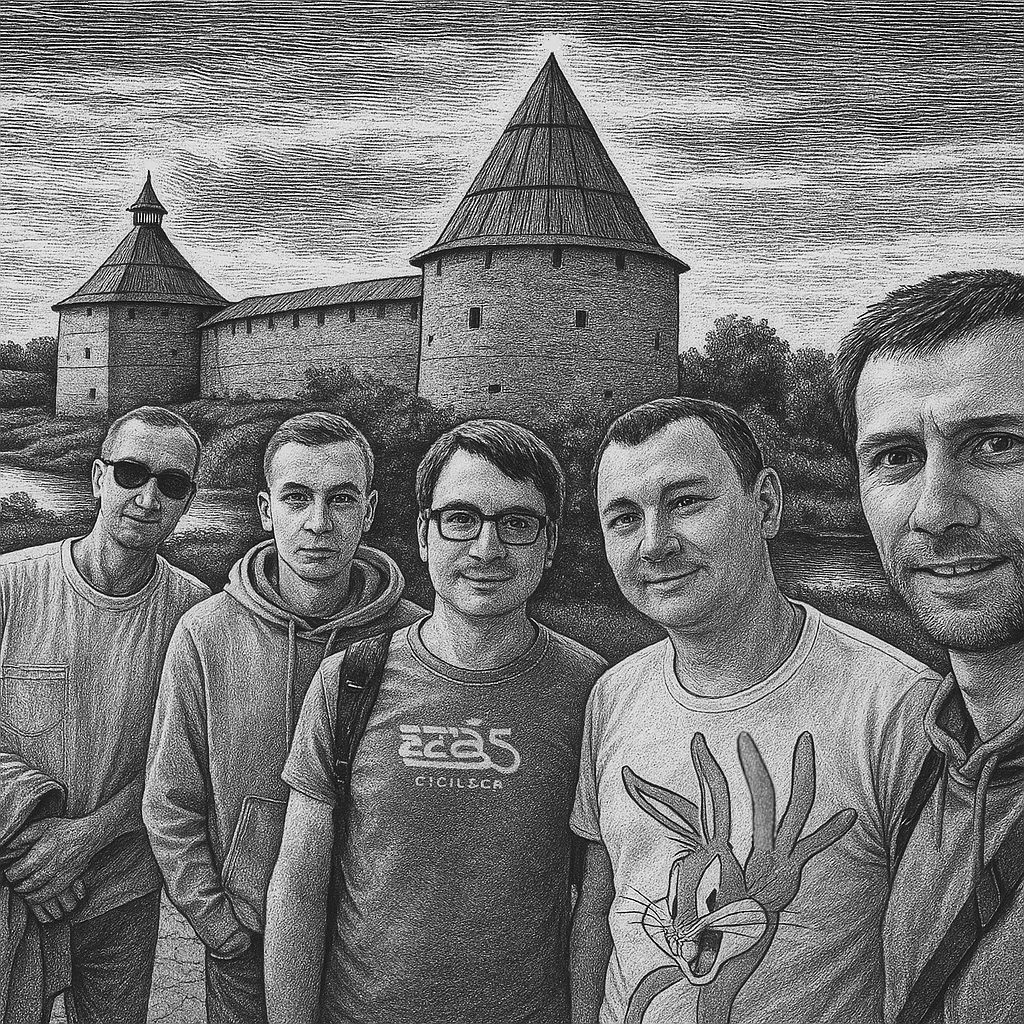
\includegraphics[width=1.0\textwidth]{60_komanda}
%	\caption{\small\textit{...упиваясь красотой местных пейзажей...}}
\end{figure}
%\end{wrapfigure}
%\vspace*{\fill}


%}

%}